\documentclass{article}
\usepackage[utf8]{inputenc}
\usepackage[margin=2cm]{geometry}
\usepackage{amsmath}
\usepackage{amssymb}
\usepackage{amsthm}
\usepackage{graphicx}
\usepackage{subfig}
\usepackage{enumitem}

\usepackage{algorithm}
\usepackage{algorithmicx}
\usepackage{algpseudocode}

\usepackage{tikz}
\usetikzlibrary{positioning}

\title{Conditional SMC genealogies}
\author{Suzie Brown\\ {\small supervised by Adam Johansen, Jere Koskela, Paul Jenkins \& Dario Span\`o}}
\date{\today}

%\usepackage[colorlinks=true, allcolors=blue]{hyperref}
\usepackage[round, sort&compress]{natbib}
\usepackage{har2nat} %%% Harvard reference style
\bibliographystyle{agsm}

\newcommand{\E}{\mathbb{E}}
\newcommand{\PR}{\mathbb{P}}
\newcommand{\V}{\operatorname{Var}}
\newcommand{\vt}[2][t]{v_{#1}^{(#2)}}
\newcommand{\vttilde}[2][t]{\tilde{v}_{#1}^{(#2)}}
\newcommand{\wt}[2][t]{w_{#1}^{(#2)}}
\newcommand{\eqdist}{\overset{d}{=}}
\newcommand{\Bin}{\operatorname{Bin}}
\newcommand{\N}{\mathcal{N}}
\newtheorem{thm}{Theorem}

\begin{document}
\maketitle

\section{Introduction}
Sequential Monte Carlo has become a popular tool, particularly in areas such as object tracking and other applications where there is a natural sequential component (usually time) and we wish to infer underlying states from noisy observations.
While these methods can be very effective for filtering, it is more difficult to apply them to smoothing because they typically suffer very badly from ancestral degeneracy in the particle genealogies.

When attempting to mitigate this problem, one often encounters a trade-off between minimising ancestral degeneracy (arising from resampling) and weight degeneracy (arising from sequential importance sampling). However, while weight degeneracy is a reasonably well-quantified problem, there exists little in the way of tools for quantifying ancestral degeneracy a priori. There are some simulation studies in the literature which attempt to cast some light on the magnitude of this problem, but analytical blah remains obscure, since the complexity of the more commonly used particle methods (those with apparently better empirical performance) makes it difficult to obtain any rigorous results.
Consequently, there is a wealth of open questions, and pertinent ones, in this area. This work attempts to extend a first result for a standard class of SMC algorithms to the case of conditional SMC with multinomial resampling. We hope this will serve as a first step towards analysing the more complex conditional SMC algorithms that are widely used in practice, particularly within the particle Gibbs algorithm.

As this work exists at the interface of sequential Monte Carlo methods and population genetics, reviews of the relevant material from both fields are summarised in Sections \ref{sec:smc} and \ref{sec:popgen} respectively. 
Section \ref{sec:previous} summarises some known results about asymptotic genealogies, both with reference to population models and particle systems.
Section \ref{sec:theory} presents the theoretical aspect of this work, which is complemented by a simulation study presented in Section \ref{sec:simulations}.

\section{Background}
\subsection{Sequential Monte Carlo}\label{sec:smc}
Although sequential Monte Carlo (SMC) methods can be applied in a much more general setting, they are particularly easy to motivate in the setting of state space models, where the ``sequential'' nature follows naturally from the discrete time steps present in the model. 
For the purposes of presenting the algorithm, let us consider a generic hidden Markov model (HMM) with hidden states $X_{0:M}$ and observables $Y_{0:M}$. We assume for notational convenience that $x_0,\dots,x_M$ take values in a common state space $\mathcal{X}$, and $y_0,\dots,y_M$ in a common state space $\mathcal{Y}$, although these assumption may readily be dropped. We will also make extensive use of the concise notation $z_{r:s} := \{z_r, z_{r+1}, \dots, z_s\}$.
\begin{align*}
& X_0 \sim \mu(\cdot) \\
& X_{t+1} \mid (X_t = x_t) \sim f(\cdot \mid x_t)  \qquad t=0,\dots,M-1 \\
& Y_t \mid (X_t = x_t) \sim g(\cdot \mid x_t) \qquad t=0,\dots,M
\end{align*}
with the conditional independence structure
\begin{align*}
& X_{t+1} \perp X_{0:t-1}, X_{t+2:M} \mid X_t \\
& Y_t \perp Y_{0:t-1}, Y_{t+1:M}, X_{0:t-1}, X_{t+1:M} \mid X_t
\end{align*}
for all $t$, as represented graphically below.

\begin{center}
\begin{tikzpicture}
\node (yt) {$Y_t$};
\node (thet) [below=of yt] {$X_t$};
\node (yt1) [left=of yt] {$Y_{t-1}$};
\node (thet1) [below=of yt1] {$X_{t-1}$};
\node (dot1) [left=of thet1] {$\dots$};
\node (dot2) [right=of thet] {$\dots$};
\draw[->](thet.north)--(yt.south);
\draw[->](thet1.north)--(yt1.south);
\draw[->](thet1.east)--(thet.west);
\draw[->](dot1.east)--(thet1.west);
\draw[->](thet.east)--(dot2.west);
\end{tikzpicture}
\end{center}

The conditional independence structure implies that the (joint) marginal distribution of the hidden states $X_{0:t}$ has the form
\begin{equation*} \label{eq:hmm_marginal}
p(x_{0:t}) = \mu(x_0) \prod_{i=1}^t f(x_i \mid x_{i-1})
\end{equation*}
and the likelihood of the observations $y_{0:t}$ given the underlying states $x_{0:t}$ has the form
\begin{equation*} \label{eq:hmm_likelihood}
p(y_{0:t} \mid x_{0:t}) = \prod_{i=0}^t g(y_i \mid x_i).
\end{equation*}

There are three main inference problems of interest in HMMs: estimating the filtering distributions $p(x_t \mid y_{0:t})$, smoothing distributions $p(x_{t} \mid y_{0:M})$ and predictive distributions $p(x_{t+1} \mid y_{0:t})$. 
The smoothing distribution $p(x_{t} \mid y_{0:M})$ is obtained from $p(x_{0:M} \mid y_{0:M})$ by marignalising. Using the conditional independence structure, we can write this distribution distributions as
\begin{align}
p(x_{0:t} \mid y_{0:t}) &\propto p(x_{0:t-1}\mid y_{0:t-1}) f(x_t\mid x_{t-1}) g(y_t \mid x_t) \label{eq:smooth_recursion}\\
&\propto \mu(x_0) g(y_0\mid x_0) \prod_{i=1}^t f(x_i \mid x_{i-1}) g(y_i\mid x_i) \notag
\end{align}
for $t = 0,\dots,M$. The filtering distribution $p(x_t \mid y_{0:t})$ can be obtained from \eqref{eq:smooth_recursion} by marginalising out $x_{0:t-1}$, which is straightforward if a Monte Carlo approximation is available.
The predictive distributions can also be derived from the smoothing distributions using
\begin{equation*}
p(x_{t+1}\mid y_{0:t}) = g(x_{t+1} \mid x_t) p(x_{0:t} \mid y_{0:t}).
\end{equation*}

SMC provides an approximation to \eqref{eq:smooth_recursion}, given a model specification and a sequence of observations. Like the underlying process, the algorithm proceeds sequentially, returning its approximation to the smoothing distribution at each time step.
A generic SMC algorithm is presented below.
\begin{algorithm}
	\caption{Standard SMC}\label{alg:SMC}
	\begin{algorithmic}[0]
    	\State \textbf{Inputs:} $\mu:\mathcal{X}\to[0,1];\quad f:\mathcal{X}\times\mathcal{X}\to[0,1];\quad g:\mathcal{Y}\times\mathcal{X}\to[0,1];\quad y_{0:M}\in\mathcal{Y}^M;\quad N\in\mathbb{N}$
		\For{$i = 1,\dots,N$}		
			\State $x_0^{(i)} \sim \mu(\cdot)$
			\State $\tilde{w}_0^{(i)} \gets g(y_0 \mid x_0^{(i)})$
			\State $w_0^{(i)} \gets \tilde{w}_0^{(i)} / \sum \tilde{w}_0^{(j)}$
		\EndFor
		\For{$t=1,\dots,M$}
        	\For{$i = 1,\dots,N$}
        		\State $\tilde{x}_t^{(i)} \gets$ {\footnotesize RESAMPLE}($\mathbf{x}_{t-1}, \mathbf{w}_{t-1}$)
				\State $x_t^{(i)} \sim f(\cdot \mid \tilde{x}_t^{(i)})$
				\State $\tilde{w}_t^{(i)} \gets g(y_t \mid x_t^{(i)})$
				\State $w_t^{(i)} \gets \tilde{w}_t^{(i)} / \sum \tilde{w}_t^{(j)}$
        	\EndFor
        \EndFor
	\end{algorithmic}
\end{algorithm}

There is a great deal of flexibility in the {\footnotesize RESAMPLE} function denoted in Algorithm \ref{alg:SMC}. The most basic choice is multinomial resampling \citep{efron1994}, but it is far from optimal in terms of estimate variance \citep{douc2005}. Various choices for the {\footnotesize RESAMPLE} function have been suggested in attempts to improve the algorithm's performance.

If only the filtering distribution is required, we can marginalise out $\mathbf{x}_{0:t-1}$ at each step by simply throwing away the particle histories and keeping only the particle approximation $\mathbf{x}_{t}$ to the filtering distribution at each time point $t$. Due to the Markovian progress of the algorithm, we only ever refer to the particles at the immediately previous step, so in this way the filtering distributions can be approximated with minimal memory usage. If, say, only the mean and variance of the filtering distribution at each time are required, we can store just these summary statistics, plus the current and previous generations of particles, and throw away all other information about the particles at previous time steps. It is also worth noting that, unlike smoothing, filtering can be carried out in an on-line fashion.

The smoothing distributions concern the full trajectories, approximated by $\mathbf{x}_{0:t}$, and it is therefore necessary in this setting to keep track of all the individual particles along with their ancestral lineages.

It is a well-studied phenomenon that SMC runs into problems when estimating smoothing distributions, because the resampling step leads to \emph{ancestral degeneracy}, whereby up to some time $m<M$ the trajectories of all particles coalesce (assuming $M$ is large enough). This is far from desirable because it means that for times $t\leq m$, the smoothing distributions $p(x_t \mid y_{0:M})$ are approximated by just one sample. Typically it is only at the last time step $p(x_M \mid y_{0:M})$ (i.e.\ the filtering distribution) that the Monte Carlo estimate consists of the full $N$ particles desired. Naturally this means that the variance in the Monte Carlo estimate blows up for $t<<M$.
%% ANCESTRAL DEGENERACY PLOT

One way to reduce the variance due to resampling is to change the {\footnotesize RESAMPLE} function.
Many people have recommended alternative sampling schemes to the basic multinomial resampling: residual resampling \citep{liu1998}, stratified resampling \citep{kitagawa1996}, systematic resampling \citep{carpenter1999} and others.

\begin{description}
\item[Multinomial resampling] New particles are sampled independently from the current set of particles $x_{t-1}^{(i)}$, with probabilities given by their weights $w_{t-1}^{(i)}$. That is, the joint distribution of the number of offspring $\mathbf{v}_{t-1} = (v_{t-1}^{(1)},\dots,v_{t-1}^{(N)})$ of the current particles is $\operatorname{Multinomial}(N, \mathbf{w}_{t-1})$.
\item[Residual resampling] Each particle $x_{t-1}^{(i)}$ is deterministically assigned $\lfloor N w_{t-1}^{(i)} \rfloor$ offspring, and the remaining $R = N- \sum \lfloor N w_{t-1}^{(i)} \rfloor$ offspring are assigned in proportion to the unaccounted-for weight. That is, $\mathbf{v}_{t-1} \eqdist \lfloor N \mathbf{w}_{t-1} \rfloor +  \operatorname{Multinomial}(R, (N \mathbf{w}_{t-1} - \lfloor N \mathbf{w}_{t-1} \rfloor)/R)$. Since part of the resampling is deterministic (and every particle with weight $>1/N$ is guaranteed to reproduce) it is intuitive that the resampling variance is mitigated.
\end{description}
Stratified and systematic resampling amount to altering the $\operatorname{U}(0,1)$ random number generator that underlies a multinomial resampling scheme.
\begin{description}
\item[Stratified resampling] Instead of sampling $N$ independent numbers from $\operatorname{U}(0,1)$, one number is sampled uniformly from each subinterval of length $1/N$, that is $U_i \sim \operatorname{U}((i-1)/N, i/N)$.
\item[Systematic resampling] Sample one random number $U \sim \operatorname{U}(0,1/N)$ and then deterministically select $N$ evenly spaced numbers $U_i = U + (i-1)/N$.
\end{description}


\citet{douc2005} presents a comparison of these three alternative resampling schemes against multinomial resampling. The authors note that of the three schemes studied, only residual resampling preserves exchangeability (as multinomial resampling does). They prove that residual and stratified sampling always yield lower variance (conditioned on all previous states) than multinomial resampling, and provide a counterexample to show that systematic resampling can sometimes perform worse than multinomial resampling. However, they concede that all three schemes seem to exhibit similar performance in practice, with systematic resampling being particularly convenient to implement.

\subsubsection{Conditional SMC}
Conditional SMC differs from the standard algorithm in that, a priori, one particular trajectory (that is, a sequence of particle positions and the corresponding ancestral line) is conditioned to survive all of the propagation and resampling steps. We will refer to this trajectory as the \emph{immortal line}, following the terminology used for conditioned Galton-Watson processes, and the \emph{immortal particle} is the particle in a particular generation that is a member of the immortal line.
This conditioning amounts to the following. We require that after a propagation step, the immortal particle ends up in its pre-conditioned position; and that after a resampling step, the immortal particle is assigned to its pre-conditioned parent.

The conditional SMC algorithm was introduced by \citet{andrieu2010} for use in particle MCMC methods. In the particle Gibbs sampler, standard SMC approximation does not admit the desired target distribution, and this problem is avoided by replacing it with a conditional SMC approximation.

A conditional SMC algorithm is summarised below. We restrict to the case of multinomial resampling since it is the simplest case in which to see the effects of condiditioning, and is the only case treated in Sections \ref{sec:theory} and \ref{sec:simulations}; for the generic algorithm see \citet[Section 4.3]{andrieu2010}. Section \ref{sec:theory} explains why the given modification to the standard multinomial resampling step is correct.
\begin{algorithm}
	\caption{Conditional SMC with multinomial resampling}\label{alg:condSMC}
	\begin{algorithmic}[0]
    	\State \textbf{Inputs:} $\mu:\mathcal{X}\to[0,1];\quad f:\mathcal{X}\times\mathcal{X}\to[0,1];\quad g:\mathcal{Y}\times\mathcal{X}\to[0,1];\quad y_{0:M}\in\mathcal{Y}^M;\quad N\in\mathbb{N}; \quad x_{0:M}^* \in \mathcal{X}^M$
    	\State $x_0^{(1)} \gets x_0^*$
    	\For{$i = 2,\dots,N$}		
			\State $x_0^{(i)} \sim \mu(\cdot)$
		\EndFor
		\For{$i = 1,\dots,N$}	
			\State $\tilde{w}_0^{(i)} \gets g(y_0 \mid x_0^{(i)})$
			\State $w_0^{(i)} \gets \tilde{w}_0^{(i)} / \sum \tilde{w}_0^{(j)}$
		\EndFor
		\For{$t=1,\dots,M$}
			\State $\tilde{x}_t^{(1)} \gets x_{t-1}^*$
			\State $x_t^{(1)} \gets x_t^*$
			\State $\tilde{\mathbf{x}}_t^{(0:N-1)} \sim \operatorname{Multinomial}(N-1, \mathbf{w}_{t-1})$
        	\For{$i = 1,\dots,N-1$}  		        		
				\State $x_t^{(i)} \sim f(\cdot \mid \tilde{x}_t^{(i)})$
			\EndFor
			\For{$i = 1,\dots,N$} 
				\State $\tilde{w}_t^{(i)} \gets g(y_t \mid x_t^{(i)})$
				\State $w_t^{(i)} \gets \tilde{w}_t^{(i)} / \sum \tilde{w}_t^{(j)}$
        	\EndFor
        \EndFor
	\end{algorithmic}
\end{algorithm}

When used as a component of the particle Gibbs algorithm, the immortal line for each iteration is sampled from the trajectories output from the previous iteration \citep[Section 2.4.3]{andrieu2010}. Thus in practice we do not have to choose the immortal line. However, for the purposes of our simulations (Section \ref{sec:simulations}), we are only studying the genealogical properties, so we do not iterate but simply perform repetitions of the conditional SMC run. In this case we have to decide on a suitable trajectory on which to condition, and the reason for our choice is detailed in Section \ref{sec:simulations}.


\subsection{Population genetics}\label{sec:popgen}
\subsubsection{Wright-Fisher model and generalisations}
One of the most popular models in population genetics is the Wright-Fisher model. Its simplifying assumptions are significant but it nonetheless seems to be useful in explaining the dynamics of genetic traits and inheritance. 
The standard model assumes a constant population size $N$, independence from one generation to the next, and exchangeability of individuals within a generation. These assumptions imply a Markov property that holds both in the forward (branching) process and the reverse (coalescent) process.

At each time step, a new generation is created by making $N$ copies of individuals from the current generation. The individuals to be copied are chosen, in the simplest case, by sampling them uniformly at random with replacement. After reproducing in this way, all individuals in the old generation die. Thus at each time step some lineages may become extinct, while others produce several copies and become more prolific.

%% wirte something about generalisations (or else change sec title). Nest site model; fertility-influencing genes. Comparison to Moran model?
%% Add example picture!!!
 
\subsubsection{Application to SMC genealogies}
The Wright-Fisher model \citep[Chapter 3]{wakeley2009}, popular in the analysis of population genetics, includes some simplifying assumptions that make it somewhat unrealistic for that application. Namely, it is assumed that the population size is constant, and that generations do not overlap. 
While these constraints may hamper the model's applicability to population genetics, it is pleasing to note that when re-purposed for the analysis of SMC genealogies, both of these rather restrictive assumptions apply automatically. At least in the most common SMC algorithms, the number of particles (population size) remains constant at each iteration, and the resampling (reproduction) procedure is applied to all particles at once.

However, a significant alteration must be made to the standard Wright-Fisher model before it can be applied to SMC. The offspring distributions of each particle are not exchangeable, because broadly speaking, offspring of parents with high weight will tend to have high weight themselves. This follows intuitively from the notion that propagating a particle from a high density region at time $t$ will result in a new state that is close to the high density region at time $t+1$.

There are generalisations of the Wright-Fisher model that do not require exchangeability among individuals, since it is also an important feature in population models. For instance, it can incorporate the existence of a hereditary trait whose value affects fertility. To model SMC genealogies, it is necessary to go one step further by allowing dependence between offspring distributions at different generations. This alteration amounts to a significant qualitative change since, while the forward process is still Markovian, the reverse (coalescent) process is not.

Whilst the population genetics literature has typically focused on the proliferation of hereditary traits \citep[Chapter 3]{wakeley2009}, our interest lies only with the genealogical process itself. The advancement of the trait, say ``being in a high density region'' is taken care of in the construction of the SMC algorithm. However, it is well-known that the problem of ``ancestral degeneracy'' is the source of much pain for practitioners; hence our interest in quantifying this problem.

\subsection{Kingman's $n$-coalescent}
\citet{kingman1982gene} introduces the \emph{$n$-coalescent} as the asymptotic genealogical process for several population models, including the Wright-Fisher model, as the population size $N\to\infty$.
In the notation of \citet{wakeley2009}, $T_i;\, i=2,\dots,n$ is the $i^{th}$ coalescence time, that is, the length of time for which there are exactly $i$ branches in the sample genealogy. The $n$-coalescent is the process in which these times are independent Exponentials:
\begin{equation*}
T_i \sim \operatorname{Exp}\left(\binom{i}{2}\right)
\end{equation*}
having
\begin{equation*}
\E(T_i) = \frac{2}{i(i-1)}, \qquad \V(T_i) = \left( \frac{2}{i(i-1)} \right)^2
\end{equation*}
By noting that the number of possible pairs from $i$ lineages is $\frac{i(i-1)}{2}$, the process can equivalently be formulated as a Poisson process where pairs of lineages coalesce independently at rate 1, with the pair to coalesce being chosen uniformly at random \citep[Section 3.2]{wakeley2009}.
\citet{mohle1998} writes the same process in terms of the infinitesimal generator $Q$ of a Markov process $\{R_r\}$ on the set of equivalence relations on $n$ elements, having entries
\begin{equation*}
q_{\xi\eta} =
\begin{cases}
-\frac{1}{2}b(b-1) &\text{if }\xi=\eta \\
1 & \text{if }\xi \prec\eta \\
0 & \text{otherwise}
\end{cases}
\end{equation*}
where $b$ is the number of equivalence classes of $\xi$, and $\xi \prec \eta$ means that $\eta$ is a state with exactly one more pair of lineages coalesced compared to $\xi$.

\subsection{Previous work}\label{sec:previous}
Kingman \citep{kingman1982gene, kingman1982coal, kingman1982exch} studied the asymptotic properties of the genealogies arising in a number of exchangeable population models, including the standard Wright-Fisher model. He showed that they each converge in the limit $N\to\infty$ (with appropriate time rescaling) to the $n$-coalescent. By studying this limiting process, he was able to establish some new results about the behaviour of such populations, and produce novel derivations of some known results.

\citet{mohle1998} extends this result to a class of non-exchangeable models, with the assumption that offspring distributions are independent between different generations. This allows application to more complex population models, such as the nest site model; but is still too restrictive to cover SMC genealogies, which by construction have strong dependence between generations.

Allowing for dependence between generations significantly complicates the computations, because the coalescent process is no longer Markovian. \citet{koskela2018} addresses a first case of such models, applicable to a range of standard SMC procedures, under some reasonable conditions.

We would like to extend to the case of conditional SMC, which differs substantially from the case of \citet{koskela2018} because there is a particular ancestral line that is conditioned to survive. This extension is important to make the results applicable to the particle Gibbs algorithm \citep{andrieu2010}, which is popular across a range of applications.

\subsubsection{Some details from the proofs}
The proofs of \citet{mohle1998} and \citet{koskela2018}, and ours by extension, rely on a decomposition of transitions into four cases.
Let $N$ be the constant population size, $v_i^{(r)}$ the (random) number of offspring in generation $r+1$ of individual $i$ in generation $r$, and let $\mathcal{R}_r$ be the equivalence relation that contains the pair $(i,j)$ iff individuals $i$ and $j$ in the last-generation sample have a common ancestor in generation $r$. 
Note that in order to maintain a constant population size the offspring numbers must satisfy
\begin{equation}\label{eq:sum_vi}
\sum_{i=1}^{M_r} v_i^{(r)} = M_{r-1}.
\end{equation}
Since particles cannot separate once coalesced, it is clear that the sequence $\{\mathcal{R}_r\}_{r \in \mathbb{N}}$ is a nested sequence of relations.
We use $\xi$ and $\eta$ to denote realisations of these relations, and consider the one-step transition mechanisms.

Let $p_{\xi\eta}(r) := \PR(\mathcal{R}_r=\eta\mid\mathcal{R}_{r-1}=\xi)$ be the one-step transition probability. Due to the aforementioned nesting, this probability is non-zero only when the equivalence classes of $\eta$ are each contained within an equivalence class of $\xi$; that is, either $\eta=\xi$ or $\eta$ is obtained from $\xi$ by merging some lineages.

A combinatorial argument allows us to derive an expression for the transition probability $p_{\xi\eta}(r)$ of the ancestral process:
\begin{equation}\label{eq:trans_prob}
p_{\xi\eta}(r) = \frac{1}{(M_{r-1})_b} \sum_{\substack{i_1,\dots,i_a =1 \\ \text{distinct}}}^{M_r} \E\left[(v_{i_1}^{(r)})_{b_1}\cdots (v_{i_a}^{(r)})_{b_a}\right]
\end{equation}
The sum is over all the possible ordered choices of the $a$ parents from generation $r$. Inside the sum is the expected number of ways to have at least the required number of offspring from each parent, given this choice of parents. Thus the whole sum represents the probability of finding a set of parents that produce the required number of offspring. Then dividing by the number of ordered ways to choose $b$ offspring from generation $r-1$ ensures that the parents produce the \emph{correct} ordered offspring. Overall then we have the probability that exactly the right subsets of offspring from generation $r-1$ coalesce in generation $r$, counting all the different parents to which they could coalesce.

We define the the \emph{coalescence probability}, i.e.\ the probability that a randomly chosen pair of (distinct) individuals from generation $r-1$ have a common ancestor in generation $r$:
\begin{equation}
c_r := \frac{1}{(M_{r-1})_2} \sum_{i=1}^{M_r} \E \left[ (v_i^{(r)})_2 \right] \label{eq:coal_prob1}
\end{equation}

We reproduce here the theorem given in \citep[Theorem 1]{mohle1998}.
We will refer to the following identities and inequalities when proving the theorem. \eqref{eq:tools_swap_sum_prod} is obtained using a multinomial expansion, \eqref{eq:tools_bernoulli_ineq} using Bernoulli's inequality, and \eqref{eq:tools_power_v_fact}--\eqref{eq:tools_fact_asymp2} by expanding factorials. 
\begin{align}
& \sum_{i_1\dots i_m = 1}^n \prod_{j=1}^m x_{i_j} = \prod_{j=1}^m \sum_{i=1}^n x_i = \left( \sum_{i=1}^n x_i \right)^m \label{eq:tools_swap_sum_prod}\\
& (k-x)^n = k^n\left(1-\frac{x}{k}\right)^n \leq k^n - nxk^{n-1} \label{eq:tools_bernoulli_ineq}\\
& n^a \geq (n)_a \label{eq:tools_power_v_fact}\\
%& (n)_a = (n)_b (n-b)_{a-b} \text{, if } 0\leq b\leq a \label{eq:tools_fact_take_two}\\
& (n)_a \leq (n)_b \,n^{a-b} \text{, if } 0\leq b\leq a \label{eq:tools_fact_taketwo_bd}\\
& \frac{n^{a-b}}{(n)_a} = \frac{1}{(n)_b} + O(n^{-b-1}) \label{eq:tools_fact_asymp1}\\
& \frac{1}{(n)_b} = \frac{1}{n^b} + O(n^{-b-1}) \label{eq:tools_fact_asymp2}
\end{align}

\begin{thm}
Let $T \subset \mathbb{R}$ and suppose there is a function $\tau : T \to \mathbb{N}_0$ satisfying:
\begin{enumerate}[label=(\Alph*)]
\item\label{assn:coal_rate} correct limiting coalescence rate
\begin{equation*}
\forall t \in T, \,\lim_{N\to\infty} \sum_{r=1}^{\tau(t)} c_r =t
\end{equation*}
\item\label{assn:coal_var} variance of coalescence rate goes to zero
\begin{equation*}
\forall t \in T, \,\lim_{N\to\infty} \sum_{r=1}^{\tau(t)} c_r^2 =0
\end{equation*}
\item\label{assn:triple_coal} no triple coalescences
\begin{equation*}
\forall t \in T, \forall k\in\mathbb{N}_0,\, \lim_{N\to\infty} \sup_{r\leq\tau(t)} \frac{1}{N^3 c_r} \sum_{i=1}^N \E\left[ (v_i^{(r)})_2 (v_i^{(r)})^k \right] =0
\end{equation*}
\item\label{assn:multi_coal} only one coalescence at a time
\begin{equation*}
\forall t \in T,\, \lim_{N\to\infty} \sup_{r\leq\tau(t)} \frac{1}{N^4 c_r} \sum_{i,j=1}^N \E\left[ (v_i^{(r)})_2 (v_j^{(r)})^2 \right] =0
\end{equation*}
\end{enumerate}
Then the finite-dimensional distributions of $\{\mathcal{R}_{\tau(t)}\}_{t\in T}$ converge to those of the $n$-coalescent (with time restricted to $T$) in the limit $N\to\infty$.
\end{thm}
Note that, since (being a probability) $c_r \geq 0$ for all $r$; under \ref{assn:coal_rate}, \ref{assn:coal_var} is equivalent to
\begin{equation}
\forall t \in T,\, \lim_{N\to\infty} \sup_{r\leq\tau(t)} c_r =0
\end{equation}

\begin{proof}
We first bound the transition probability $p_{\xi\eta}(r)$ as given by \eqref{eq:trans_prob}, in each of four possible cases. This will show that the only type of coalescence event to occur at any one time in the limit $N\to\infty$ is a merger of exactly one pair of lineages (\ref{case:pair_merge} below). 
Assume the offspring numbers $v_i^{(r)}$ are known (so we drop the expectations).
\begin{enumerate}[label = \textbf{Case \arabic*.}]
\item\label{case:pair_merge} $\eta$ is obtained from $\xi$ by merging exactly one pair of lineages, i.e.\ $b_1=2, b_2=\dots=b_a=1$, and $b=a+1$. We derive an upper bound:
\begin{align}
p_{\xi\eta}(r) &= \frac{1}{(N)_b} \sum_{\substack{i_1,\dots,i_a =1 \\ \text{distinct}}}^{N} (v_{i_1}^{(r)})_2(v_{i_2}^{(r)})_1\cdots (v_{i_a}^{(r)})_1 &\notag\\
&\leq \frac{1}{(N)_b} \sum_{i_1,\dots,i_a=1}^N (v_{i_1}^{(r)})_2 (v_{i_2}^{(r)})_1 \cdots (v_{i_a}^{(r)})_1 &\text{dropping distinctness} \notag\\
&= \frac{1}{(N)_b} \sum_{i=1}^N (v_i^{(r)})_2 \sum_{i_2,\dots,i_a=1}^N v_{i_2}^{(r)} \cdots v_{i_a}^{(r)} & \notag\\
&= \frac{1}{(N)_b} \sum_{i=1}^N (v_i^{(r)})_2 (v_1^{(r)} + \dots + v_N^{(r)})^{a-1} & \text{using \eqref{eq:tools_swap_sum_prod}} \notag\\
&= \frac{N^{b-2}}{(N)_b} \sum_{i=1}^N (v_i^{(r)})_2 & \text{using \eqref{eq:sum_vi}} \notag\\
&= \left( \frac{1}{(N)_2} + O(N^{-3}) \right) \sum_{i=1}^N (v_i^{(r)})_2 & \text{using \eqref{eq:tools_fact_asymp1}} \label{eq:case1_upper}\\
&= c_r + o(c_r) & \text{by \eqref{eq:coal_prob1} and \ref{assn:triple_coal}} \notag
\end{align}
and a lower bound:
\begin{align}
p_{\xi\eta}(r) &= \frac{1}{(N)_b} \sum_{\substack{i_1,\dots,i_a =1 \\ \text{distinct}}}^{N} (v_{i_1}^{(r)})_2(v_{i_2}^{(r)})_1\cdots (v_{i_a}^{(r)})_1 &\notag\\
&= \frac{1}{(N)_b} \sum_{i=1}^N (v_i^{(r)})_2 \sum_{\substack{i_2,\dots,i_a =1 \\ \text{distinct} \neq i }}^{N} (v_{i_2}^{(r)})_1\cdots (v_{i_a}^{(r)})_1 &\notag\\
&\geq \frac{1}{(N)_b} \sum_{i=1}^N (v_i^{(r)})_2 \sum_{j\neq i} \sum_{\substack{i_3,\dots,i_a\\ \neq i}}\left[ v_j\cdot v_{i_3}\cdots v_{i_a} - \binom{b-2}{2}(v_j^{(r)})^2 \cdot v_{i_4}\cdots v_{i_a} \right] & \label{eq:transprob_lowerbd}\\
&= \frac{1}{(N)_b} \sum_{i=1}^N (v_i^{(r)})_2 \left[ \sum_{i_2,\dots,i_a\neq i} v_{i_2}\cdots v_{i_a} - \binom{b-2}{2} \sum_{i_3,\dots,i_a\neq i} v_{i_3}\cdots v_{i_a} \sum_{j \neq i} (v_j^{(r)})^2 \right] & \notag\\
&= \frac{1}{(N)_b} \sum_{i=1}^N (v_i^{(r)})_2 \left[ (N-v_i)^{b-2} - \binom{b-2}{2} \sum_{j\neq i} (v_j^{(r)})^2 N^{b-4} \right] &\text{using \eqref{eq:tools_swap_sum_prod}} \notag\\
&= \frac{1}{(N)_b} \sum_{i=1}^N (v_i^{(r)})_2  (N-v_i)^{b-2} - \frac{1}{(N)_b} \binom{b-2}{2} \sum_{i\neq j=1}^{N} (v_i^{(r)})_2 (v_j^{(r)})^2 N^{b-4} & \notag\\
&\geq \frac{1}{(N)_b} \sum_{i=1}^N (v_i^{(r)})_2  (N)^{b-2} - \frac{1}{(N)_b}(b-2)\sum_{i=1}^{N} (v_i^{(r)})_2 v_i^{(r)} N^{b-3} \notag\\
&\phantom{=\qquad\qquad} - \frac{1}{(N)_b}\binom{b-2}{2} \sum_{i\neq j=1}^{N} (v_i^{(r)})_2 (v_j^{(r)})^2 N^{b-4} &\text{using \eqref{eq:tools_bernoulli_ineq}} \notag\\
&\geq \frac{1}{(N)_2} \sum_{i=1}^N (v_i^{(r)})_2 - \frac{(b-2)N^{b-3}}{(N)_b}\sum_{i=1}^{N} (v_i^{(r)})_2 v_i^{(r)} \notag\\
&\phantom{=\qquad\qquad} -\frac{N^{b-4}}{(N)_b}\binom{b-2}{2} \sum_{i\neq j=1}^{N} (v_i^{(r)})_2 (v_j^{(r)})^2 & \notag\\
&= \frac{1}{(N)_2} \sum_{i=1}^N (v_i^{(r)})_2 - \left[\frac{(b-2)}{N^3} +O(N^{-4}) \right] \sum_{i=1}^{N} (v_i^{(r)})_2 v_i^{(r)} \notag\\
&\phantom{=\qquad\qquad} -\left[ \frac{1}{N^4}\binom{b-2}{2} + O(N^{-5}) \right] \sum_{i\neq j=1}^{N} (v_i^{(r)})_2 (v_j^{(r)})^2 &\text{using \eqref{eq:tools_fact_asymp1}, \eqref{eq:tools_fact_asymp2}} \\
&= c_r + o(c_r) &\text{by \eqref{eq:coal_prob1},\ref{assn:triple_coal},\ref{assn:multi_coal}} \notag
\end{align}
Hence in this case $p_{\xi\eta}(r)=c_r +o(c_r)$.
The inequality \eqref{eq:transprob_lowerbd} is obtained by bounding the number of configurations with distinct parents by the the number of configurations with not necessarily distinct parents minus the number with at least one pair of parents chosen indistinctly. This leaves us with only the distinct-parents configurations since all indistinct choices must necessarily have a pair of parents chosen indistinctly, and the inequality arises from double-counting.

\item\label{case:triple_merge} $\eta$ is obtained from $\xi$ by merging three or more lineages into one, possibly as well as other simultaneous mergers, i.e.\ $b_1\geq3$.
\begin{align}
p_{\xi\eta}(r) &= \frac{1}{(N)_b} \sum_{\substack{i_1,\dots,i_a =1 \\ \text{distinct}}}^{N} (v_{i_1}^{(r)})_{b_1}(v_{i_2}^{(r)})_{b_2}\cdots (v_{i_a}^{(r)})_{b_a} &\notag\\
&\leq \frac{1}{(N)_b} \sum_{i=1}^{N} (v_{i}^{(r)})_{b_1} \sum_{i_2,\dots,i_a =1}^{N} (v_{i_2}^{(r)})_{b_2}\cdots (v_{i_a}^{(r)})_{b_a} &\notag\\
&\leq \frac{1}{(N)_b} \sum_{i=1}^{N} (v_{i}^{(r)})_{b_1} (v_1^{(r)}+\dots+v_a^{(r)})^{b_2+\dots+b_a} &\text{using \eqref{eq:tools_swap_sum_prod}} \notag\\
&\leq \frac{1}{(N)_b} \sum_{i=1}^{N} (v_{i}^{(r)})_{b_1} N^{b-3} &\text{since }b_2+\dots+b_a\leq b-3 \label{eq:triplemerge_bound_spinoff}\\
%%^ HAVE TO SPIN OFF HERE FOR KJJS PROOF
&\leq \frac{N^{b-3}}{(N)_b} \sum_{i=1}^{N} (v_{i}^{(r)})_{2}(v_{i}^{(r)})^{b_1-2}  &\text{using \eqref{eq:tools_fact_taketwo_bd}} \\
&= o(c_r) &\text{using \ref{assn:triple_coal}} \notag
\end{align}

\item\label{case:multi_merge} $\eta$ is obtained from $\xi$ via two or more pair mergers, with no merges of more than two lineages, i.e.\ $2=b_1=b_2\geq b_3\geq\dots\geq b_a\geq1$.
\begin{align}
p_{\xi\eta}(r) &= \frac{1}{(N)_b} \sum_{\substack{i_1,\dots,i_a =1 \\ \text{distinct}}}^{N} (v_{i_1}^{(r)})_2 (v_{i_2}^{(r)})_2 (v_{i_3}^{(r)})_{b_3}\cdots (v_{i_a}^{(r)})_{b_a} &\notag\\
&\leq \frac{1}{(N)_b} \sum_{i=1}^{N} (v_{i}^{(r)})_2 \sum_{j=1}^N (v_j^{(r)})_2 \sum_{i_3,\dots,i_a =1}^{N} (v_{i_3}^{(r)})_{b_3}\cdots (v_{i_a}^{(r)})_{b_a} &\text{dropping distinctness}\notag\\
&\leq \frac{1}{(N)_b} \sum_{i=1}^{N} (v_{i}^{(r)})_2 \sum_{j=1}^N (v_j^{(r)})^2 \sum_{i_3,\dots,i_a =1}^{N} (v_{i_3}^{(r)})_{b_3}\cdots (v_{i_a}^{(r)})_{b_a} &\text{using \eqref{eq:tools_power_v_fact}} \notag\\
&\leq \frac{1}{(N)_b} \sum_{i,j=1}^{N} (v_{i}^{(r)})_2 (v_j^{(r)})^2 (v_1^{(r)}+\dots+v_N^{(r)})^{b_3+\dots +b_a} &\notag\\
&=\frac{N^{b-4}}{(N)_b} \sum_{i,j=1}^N (v_{i}^{(r)})_2 (v_j^{(r)})^2 & \\
&= o(c_r) &\text{using \ref{assn:multi_coal}} \notag
\end{align}

\item\label{case:no_change} $\eta=\xi$, i.e.\ $b_1=\dots=b_a=1$, and $a=b$.
\begin{align}
p_{\xi\xi}(r) &= \frac{1}{(N)_a} \sum_{\substack{i_1,\dots,i_a =1 \\ \text{distinct}}}^{N} (v_{i_1}^{(r)})_1  \cdots (v_{i_a}^{(r)})_1 & \notag\\
&= \frac{1}{(N)_a} \sum_{\substack{i_1,\dots,i_a =1 \\ \text{distinct}}}^{N} v_{i_1}^{(r)} \cdots v_{i_a}^{(r)} & \notag\\
&= \frac{1}{(N)_a} \left[ \sum_{i_1,\dots,i_a =1}^N v_{i_1}^{(r)} \cdots v_{i_a}^{(r)} - \binom{a}{2}\sum_{j=1}^N (v_j^{(r)})^2 \sum_{i_3,\dots,i_a =1}^N v_{i_3}^{(r)} \cdots v_{i_a}^{(r)} \right] &\label{eq:transprob_lowerbd2}\\
&= \frac{1}{(N)_a} \left[ (v_1^{(r)}+\dots+v_N^{(r)})^a - \binom{a}{2} \sum_{i=1}^N (v_i^{(r)})^2 (v_1^{(r)}+\dots+v_N^{(r)})^{a-2} \right] &\text{using \eqref{eq:tools_swap_sum_prod}} \notag\\
&= \frac{1}{(N)_a} \left[ N^a - \binom{a}{2} N^{a-2} \sum_{i=1}^N (v_i^{(r)})^2 \right] &\notag\\
&\geq 1- \binom{a}{2} \frac{N^{a-2}}{(N)_a} \sum_{i=1}^N (v_i^{(r)})^2 &\text{using \eqref{eq:tools_power_v_fact}}\notag\\
%&= 1- \binom{a}{2} \frac{N^{a-2}}{(N)_2 (N-2)_{a-2}} \sum_{i=1}^N (v_i^{(r)})^2 &\text{using \eqref{eq:tools_fact_take_two}}\notag\\
&= 1- \binom{a}{2} \left[ \frac{1}{(N)_2} + O(N^{-3}) \right] \sum_{i=1}^N (v_i^{(r)})^2 &\text{using \eqref{eq:tools_fact_asymp1}}\\
&= 1- c_r +o(c_r) &\notag
\end{align}
\end{enumerate}
The equality \eqref{eq:transprob_lowerbd2} is obtained in the same way as \eqref{eq:transprob_lowerbd}, with no double-counting.
We have now shown that the only coalescence events having positive probability in the limit $N\to\infty$ are staying the same (\ref{case:no_change}) or merging a single pair of lineages (\ref{case:pair_merge}). All other possibilities have asymptotic probability $o(c_r)$.

It remains to show that the finite-dimensional distributions converge to those of the Kingman coalescent. Because the processes considered are Markov even when viewed as coalescing backwards in time, it suffices to show that the generators of the process converge to the generators of the Kingman coalescent (this will no longer be the case for the processes considered in \citet{koskela2018}).
\end{proof}

For the argument of \citet{koskela2018}, a different form is needed for the upper bound on triple mergers (\ref{case:triple_merge}). Starting from \eqref{eq:triplemerge_bound_spinoff}, we obtain:
\begin{align}
p_{\xi\eta}(r) &\leq \frac{1}{(N)_b} \sum_{i=1}^{N} (v_{i}^{(r)})_{b_1} N^{b-3} \notag\\
&\leq \frac{N^{b-3}}{(N)_b} \sum_{i=1}^{N} (v_{i}^{(r)})^{b_1} \notag\\
&= \left[ \frac{1}{N^3} + O(N^{-4}) \right] \sum_{i=1}^{N} (v_{i}^{(r)})^{b_1}
\end{align}


\section{Theoretical results}\label{sec:theory}
We now consider extending the results of \citet{koskela2018} to the case of conditional SMC.
Here the SMC updates are conditioned on a particular trajectory surviving. We concentrate on the exchangeable model, so we may take without loss of generality that the ``immortal line'' is the trajectory containing individual 1 from each generation.
We first assume the simplest case, with multinomial resampling (see Algorithm \ref{alg:condSMC}); which is analogous to the standard SMC case where
\begin{equation*}
\vt{i} \eqdist \Bin (N, \wt{i}), \qquad i=1,\dots,N
\end{equation*}
yielding the coalescence rate
\begin{equation}
c_N(t) := \frac{1}{(N)_2} \sum_{i=1}^{N} \E\left[ (\vt{i})_2 \right] = \sum_{i=1}^{N} \E\left[(\wt{i})^2\right].
\end{equation}
But now, since the first line is immortal, in each time step the first individual must have at least one offspring. The remaining $N-1$ offspring are assigned multinomially to the $N$ possible parents as usual, giving the offspring numbers:
\begin{align*}
& \vttilde{1} \eqdist 1 + \Bin(N-1, \wt{1}) \\
& \vttilde{i} \eqdist \Bin(N-1, \wt{i}), \qquad i=2,\dots,N.
\end{align*}
We therefore have the following moments (using tower property):
\begin{align*}
& \E[\vttilde{i}] = (N-1)\E[\wt{i}] &\\
& \E[(\vttilde{i})^2] = (N-1)(N-2)\E[(\wt{i})^2] + (N-1)\E[\wt{i}] &\qquad i=2,\dots,N \\
& \E[\vttilde{1}] = (N-1)\E[\wt{1}] + 1 \\
& \E[(\vttilde{1})^2] = (N-1)(N-2)\E[(\wt{1})^2] + 3(N-1)\E[\wt{1}] + 1 &
\end{align*}
and we can derive the altered coalescence rate:
\begin{align}
\tilde{c}_N(t) &= \frac{1}{(N)_2} \sum_{i=1}^{N} \E\left[ (\vttilde{i})_2 \right] \notag\\
&= \frac{1}{(N)_2} \E\left[ (\vttilde{1})^2 - \vttilde{1} \right] + \frac{1}{(N)_2}\sum_{i=2}^{N} \E\left[ (\vttilde{i})^2 - \vttilde{i} \right] \notag\\
&= \frac{1}{(N)_2}\left[ (N-1)(N-2)\E[(\wt{1})^2] + 2(N-1)\E[\wt{1}] \right] + \frac{1}{(N)_2} \sum_{i=2}^{N} (N-1)(N-2)\E[(\wt{i})^2] \notag\\
&= \frac{1}{(N)_2} \sum_{i=1}^{N} (N-1)(N-2)\E[(\wt{i})^2] + \frac{1}{(N)_2} 2(N-1)\E[\wt{1}] \notag\\
&= \frac{N-2}{N} c_N(t) + \frac{2}{N} \E[\wt{1}]
%&\overset{N\to\infty}{\longrightarrow} c_N(t) \notag
\end{align}
%Since $\wt{1} \leq 1$ for all $t$, as $N\to\infty$ we have
%\begin{equation*}
%\tilde{c}_N(t) - c_N(t) = O(N^{-1}).
%\end{equation*}
Under the conditions of \citet[Corollary 2]{koskela2018}, we have that $\E[\wt{1}] = O(N^{-1})$, and hence
\begin{equation*}
\tilde{c}_N(t) - c_N(t) = O(N^{-2}).
\end{equation*}
%\begin{equation*}
%\tilde{c}_N(t) = \frac{N-2}{N} c_N(t) + O(N^{-2}) = c_N(t) + O \left( \frac{c_N(t)}{N} \right)
%\end{equation*}
\citet{koskela2018} gives the following bounds on $c_N(t)$:
\begin{equation*}
\frac{C_*}{N-1} \leq c_N(t) \leq \frac{C}{N-1}
\end{equation*}
Then, since $\tilde{c}_N(t)$ differs from $c_N(t)$ by $O(N^{-2})$, for sufficiently large $N$ there exist constants $\tilde{C}, \tilde{C}_*$ such that
\begin{equation*}
\frac{\tilde{C}_*}{N-1} \leq \tilde{c}_N(t) \leq \frac{\tilde{C}}{N-1}
\end{equation*}
and we can thus derive bounds analogous to \citet[(5)-(6)]{koskela2018}:
\begin{align}
\frac{N-1}{\tilde{C}_*}t &\leq \tilde{\tau}_N(t) \leq \frac{N-1}{\tilde{C}}t \label{eq:tau_bounds1}\\
\frac{N-1}{\tilde{C}_*}(s-t) &\leq \tilde{\tau}_N(s) - \tilde{\tau}_N(t) \leq \frac{N-1}{\tilde{C}}(s-t) \label{eq:tau_bounds2}
\end{align}
Furthermore, we have that
\begin{align*}
\frac{\tilde{C}}{N-1} &= \frac{N-2}{N} \frac{C}{N-1} + O(N^{-2}) \\
&= \frac{C}{N-1} + O(N^{-2})
\end{align*}
therefore $\tilde{C} - C = O(N^{-1})$ and similarly $\tilde{C}_* - C_* = O(N^{-1})$. Hence the bounds in \eqref{eq:tau_bounds1}, \eqref{eq:tau_bounds2} are asymptotically equal to those of \citet[(5)--(6)]{koskela2018}.

It remains to verify that the conditions \citep[(3)--(4)]{koskela2018} can extend to this case. If so, a modified version of \citet[Theorem 1]{koskela2018} and its corollaries will hold, by the same argument, for conditional SMC.

\section{Simulation study}\label{sec:simulations}
In order to investigate how well the asymptotic results hold for finite $N$, we conducted a simulation study on the Ornstein-Uhlenbeck model, a ``simplest case'' hidden Markov model which is popular for such studies in the literature:
\begin{align*}
& X_0 \sim \N(0,1) \\
& X_{t+1} \mid X_t \sim \N((1-\Delta)X_t, \Delta) \\
& Y_t \mid X_{t} \sim \N(X_t, \sigma^2)
\end{align*}
with parameters $\Delta >0, \sigma >0$.

Tree height $T$ is one of the basic properties of an ancestral sub-tree. It denotes the number of generations back one must go to find the most recent common ancestor (MRCA) of a sample of $n$ leaves (individuals from generation $N_{obs}$). That is, how many time steps of the reverse process pass before the $n$ sampled lineages all coalesce to a single lineage. If the asymptotic genealogical process is known to be an $n$-coalescent, moments of $T$ are available analytically. In particular, we expect for conditional SMC to obtain the same limiting process as for standard SMC, since we have shown in Section [REF] that their coalescent rates are asymptotically equal. Therefore in the limit as $N\to\infty$ we expect the moments of $T$ to behave as stated in \citet[Corollary 1]{koskela2018}:
\begin{align*}
\frac{C_*}{C^2} \left(1-\frac{1}{n}\right) + O(N^{-1}) &\leq \E[T/N] \leq 2\frac{C}{C_*^2} \left(1-\frac{1}{n}\right) \\
\left(\frac{4\pi^2}{3} - 12 + O(n^{-1})\right) \left(\frac{C_*}{C^2}\right)^2 + O(N^{-1}) &\leq \V(T/N) \leq \left(\frac{4\pi^2}{3} - 12 + O(n^{-1})\right) \left(\frac{C}{C_*^2}\right)^2
\end{align*}
where of course $T$ depends on $n$ and $N$. In particular, the choice of immortal line does not feature in these bounds and so should have no effect as $N \to\infty$ with respect to $n$.

Following \citet{koskela2018}, we take $\Delta = \sigma = 0.1$ and generate one fixed sequence of observations for use in all SMC runs.
We use a range of values $\{256, 512, \dots, 4096\}$ for $N$, and two fixed values $n=2,16$ intended to show the qualitative difference in behaviour as we cross a supposed ``$n<<N$'' threshold.
The number of observations $N_{obs}$ is taken such that, for all the choices of $n$ and $N$, the $N_{obs}$ generations of SMC particles are enough for the $n$ sampled lineages to coalesce to one common ancestor (with high enough probability that it happens reliably on every repetition); ensuring that the tree height can always be recorded.

For this toy model, the smoothing distribution is available analytically through the Rauch-Tung-Striebel (RTS) smoother \citep{rauch1965}. We exploited this solution to choose the ``immortal line'' on which to condition the conditional SMC updates. Because both the MAP estimate (equal to the mean since the distributions are Gaussian) and variance are available via the RTS smoother, we were able to produce a sequence of immortal lines of decreasing likelihood, by adding multiples of the standard deviation to the mean.

We hypothesised that when $N$ is not too much bigger than $n$, an ``unlikely'' choice of the immortal line should produce qualitative differences in the tree height profile; because the$n$ lineages would often coalesce to the immortal line, which corresponds to an unlikely choice of ancestors under the unconditional algorithm. On the other hand, when $N$ is very large with respect to $n$, this effect should become less significant because the sampled lineages should usually coalesce before interacting with the immortal line.

Figures \ref{fig:kalman_n16} and \ref{fig:kalman_n2} illustrate this distinction. Here we use a decrease in $n$ as a proxy for increasing $N$: over the same range of values for $N$, Figure \ref{fig:kalman_n16} shows the profile for sample size $n=16$, and Figure \ref{fig:kalman_n2} for $n=2$.
We see clearly that in the case of $n=16$, the likelihood of the immortal line significantly affects the tree height profile, while for $n=2$ it makes no appreciable difference.

In any case the mean tree height seems to be higher for conditional SMC (around 0.3) compared to standard SMC (around 0.2), although it is not yet entirely clear.

\begin{figure}
\centering
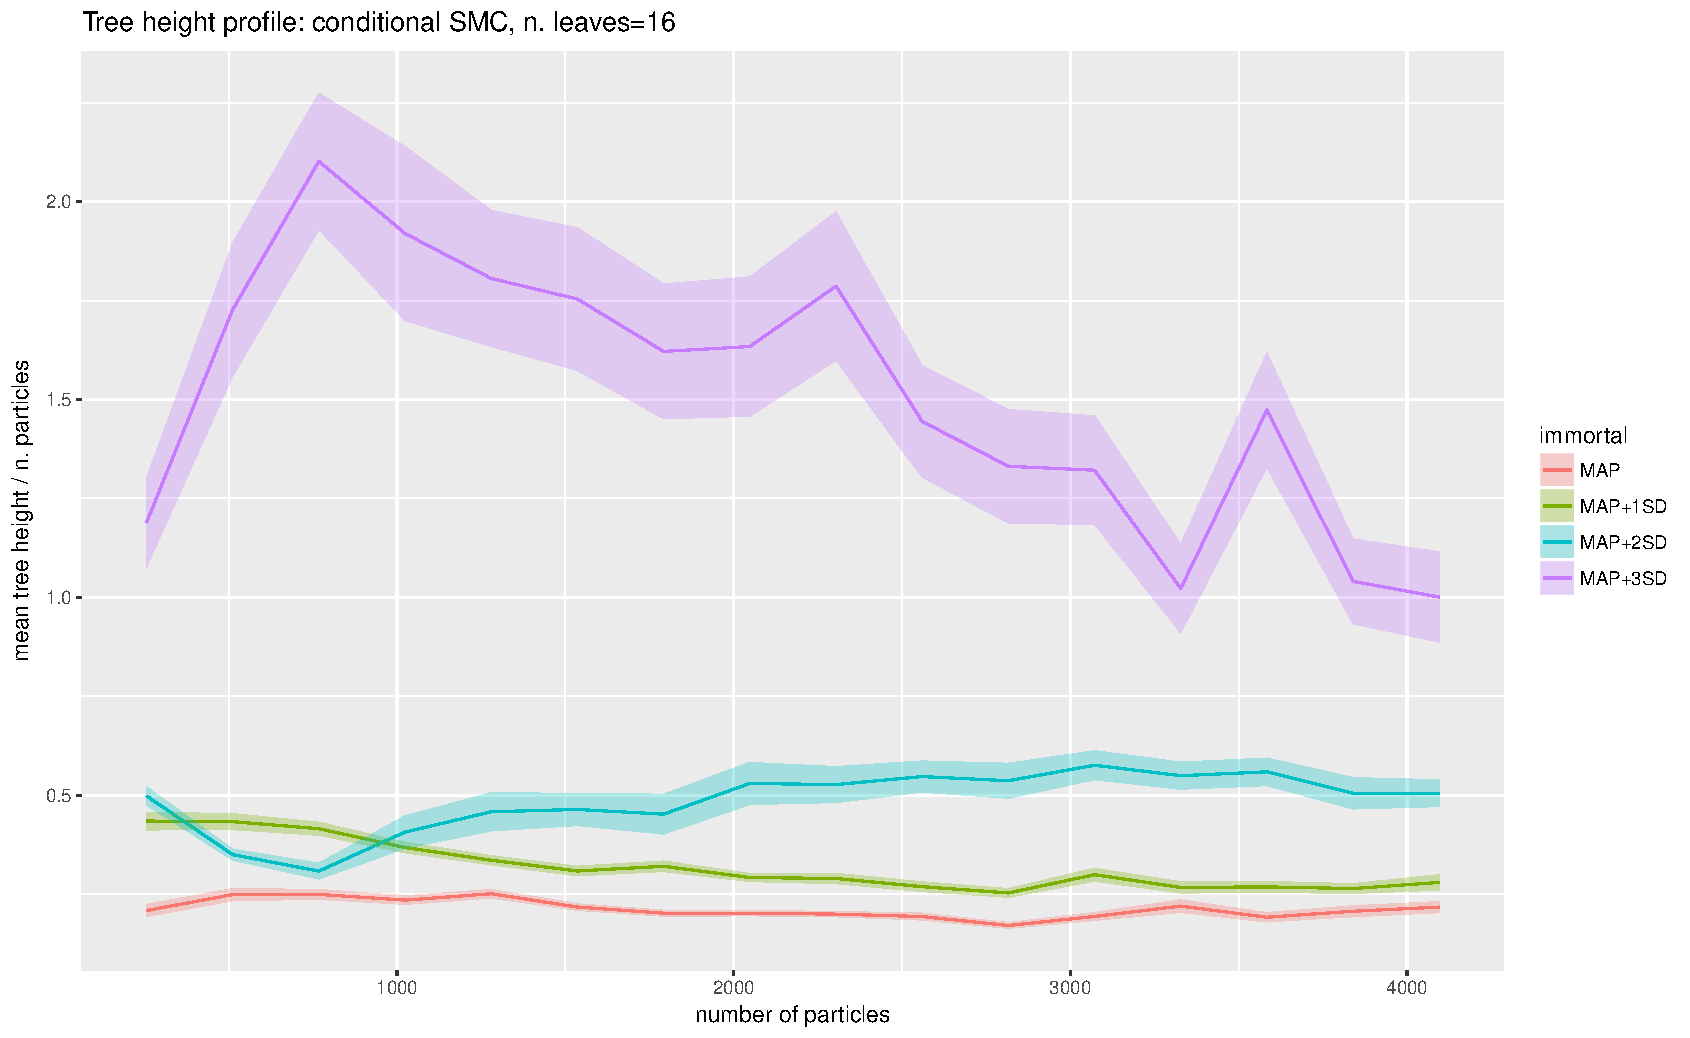
\includegraphics[width=\textwidth]{kalman_n16_100reps_line.pdf}
\caption{$\E(T/N)$ for samples of $n=16$ leaves from conditional SMC where the immortal line is 0,1,2,3 standard deviations away from the MAP estimate. Each point is averaged over 100 repetitions of running the particle filter and sampling $n$ leaves; and the same sequence of observations was used for every run. Different choices of immortal line clearly have a profound effect on tree height: in the number of generations taken for 16 lineages to coalesce, it is likely that the subtree will contain part of the immortal line.}
\label{fig:kalman_n16}
\end{figure}
\begin{figure}
\centering
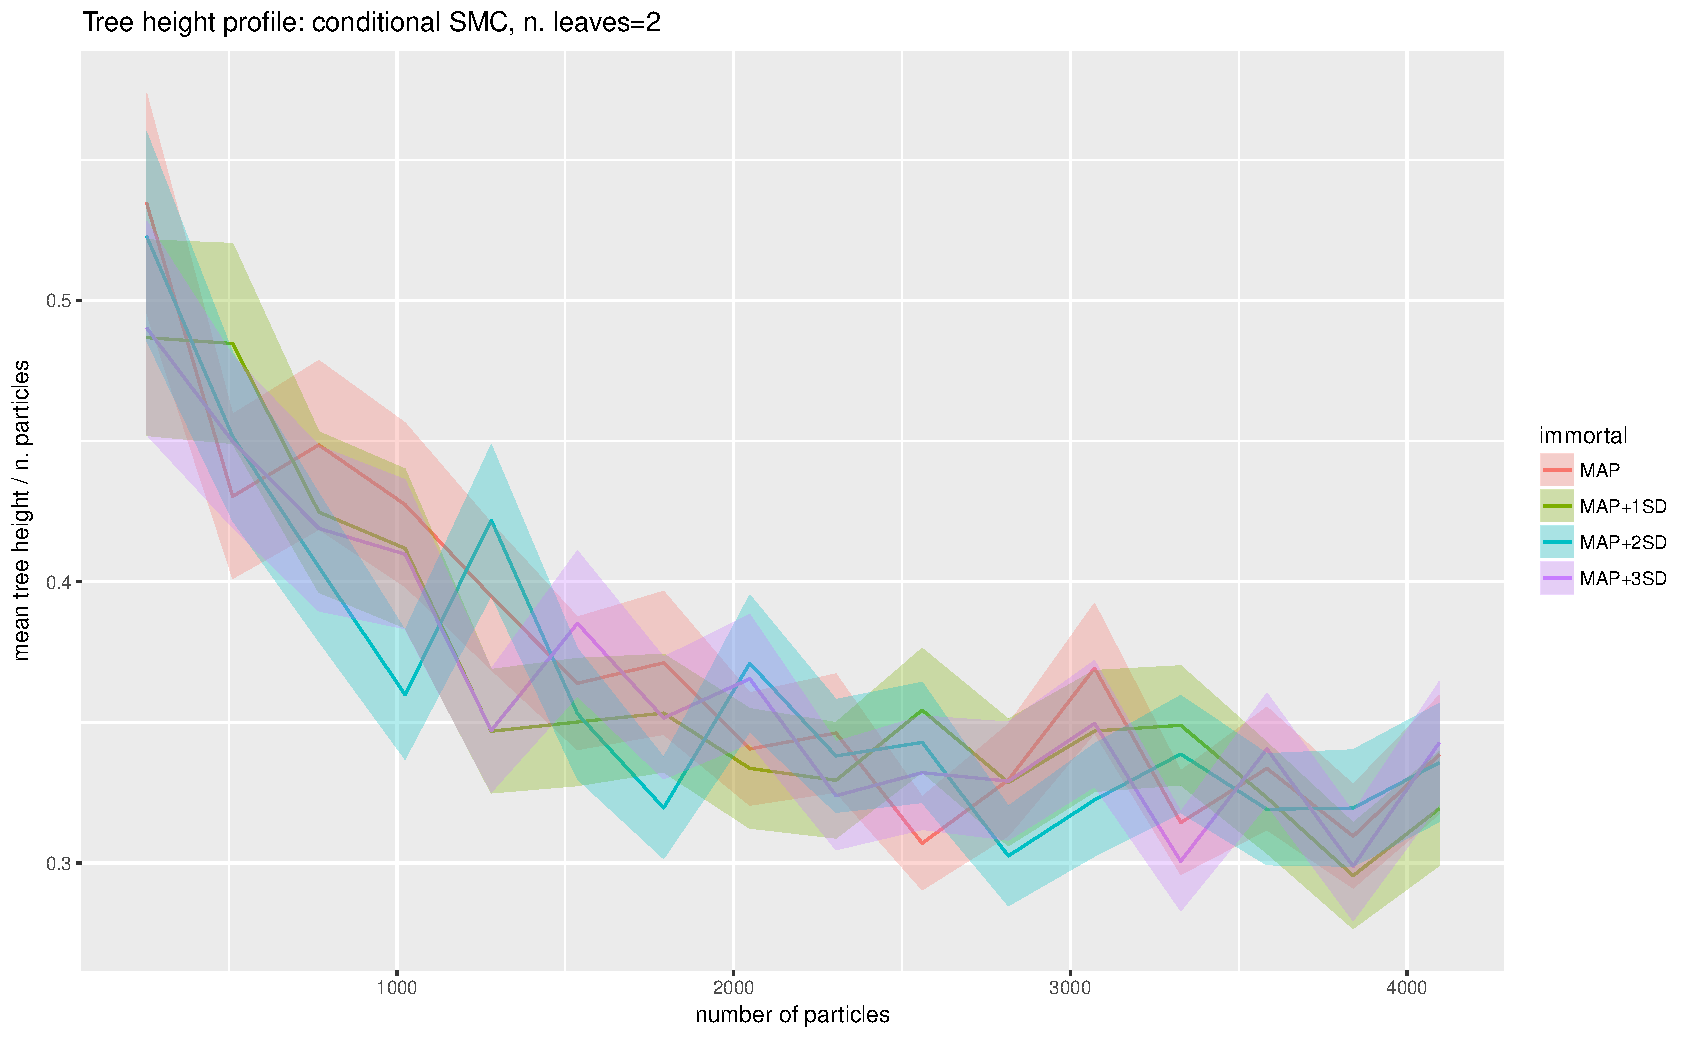
\includegraphics[width=\textwidth]{kalman_n2_1000reps_line.pdf}
\caption{$\E(T/N)$ for samples of $n=2$ leaves from conditional SMC where the immortal line is 0,1,2,3 standard deviations away from the MAP estimate. Each point is averaged over 1000 repetitions of running the particle filter and sampling $n$ leaves; and the same sequence of observations was used for every run. Now the choice of immortal line does not seem to affect the tree height: $n$ is so small compared to $N$  that it is unlikely to sample a pair of lineages that meet the immortal line before coalescing.}
\label{fig:kalman_n2}
\end{figure}

\section{Conclusions}
We have showed that under multinomial resampling, the coalescence probability for conditional SMC is close enough to that of standard SMC to imply the existence of a time rescaling that is asymptotically equivalent to that defined in \citet[p.7]{koskela2018}. Given this result, we expect their result to be transferable to the conditional SMC setting, although conditions \citet[(3)--(4)]{koskela2018} still need to be verified.

While \citet[Section 3]{koskela2018} demonstrates that in the case of standard SMC, the asymptotic results seem to hold even for $n=N$, we conclude from the simulation study that the asymptotic results for conditional SMC will require $n << N$.
Although we have demonstrated empirically that $n <<N$ is required to mitigate the effect of choosing an unlikely immortal line, this in itself should not raise concerns with those implementing the particle Gibbs algorithm. In particle Gibbs, the immortal line is sampled from the trajectories generated in the previous iteration, proportionally to their likelihood. Unless all the generated trajectories are unlikely (in which case there are more profound problems with the algorithm), the immortal line will therefore usually be a reasonably likely one.

We expect that less straight-forward conditional SMC algorithms, using alternative resampling schemes, should have the same limiting genealogical process (up to constants) as the multinomial scheme; as was hypothesised and demonstrated empirically in \citet{koskela2018} for standard SMC. Proving this even for standard SMC remains an open problem.
There are many other directions for generalising these results, in particular investigating their robustness under violation of the various assumptions, either theoretically or empirically. It is of particular interest to consider the classes of SMC algorithms most often used in practice. It was to this end that we began looking at conditional SMC, since the particle Gibbs algorithm is widely used in numerous applications.

\bibliography{smc.bib}
\end{document}